\documentclass[1p]{elsarticle_modified}
%\bibliographystyle{elsarticle-num}

%\usepackage[colorlinks]{hyperref}
%\usepackage{abbrmath_seonhwa} %\Abb, \Ascr, \Acal ,\Abf, \Afrak
\usepackage{amsfonts}
\usepackage{amssymb}
\usepackage{amsmath}
\usepackage{amsthm}
\usepackage{scalefnt}
\usepackage{amsbsy}
\usepackage{kotex}
\usepackage{caption}
\usepackage{subfig}
\usepackage{color}
\usepackage{graphicx}
\usepackage{xcolor} %% white, black, red, green, blue, cyan, magenta, yellow
\usepackage{float}
\usepackage{setspace}
\usepackage{hyperref}

\usepackage{tikz}
\usetikzlibrary{arrows}

\usepackage{multirow}
\usepackage{array} % fixed length table
\usepackage{hhline}

%%%%%%%%%%%%%%%%%%%%%
\makeatletter
\renewcommand*\env@matrix[1][\arraystretch]{%
	\edef\arraystretch{#1}%
	\hskip -\arraycolsep
	\let\@ifnextchar\new@ifnextchar
	\array{*\c@MaxMatrixCols c}}
\makeatother %https://tex.stackexchange.com/questions/14071/how-can-i-increase-the-line-spacing-in-a-matrix
%%%%%%%%%%%%%%%

\usepackage[normalem]{ulem}

\newcommand{\msout}[1]{\ifmmode\text{\sout{\ensuremath{#1}}}\else\sout{#1}\fi}
%SOURCE: \msout is \stkout macro in https://tex.stackexchange.com/questions/20609/strikeout-in-math-mode

\newcommand{\cancel}[1]{
	\ifmmode
	{\color{red}\msout{#1}}
	\else
	{\color{red}\sout{#1}}
	\fi
}

\newcommand{\add}[1]{
	{\color{blue}\uwave{#1}}
}

\newcommand{\replace}[2]{
	\ifmmode
	{\color{red}\msout{#1}}{\color{blue}\uwave{#2}}
	\else
	{\color{red}\sout{#1}}{\color{blue}\uwave{#2}}
	\fi
}

\newcommand{\Sol}{\mathcal{S}} %segment
\newcommand{\D}{D} %diagram
\newcommand{\A}{\mathcal{A}} %arc


%%%%%%%%%%%%%%%%%%%%%%%%%%%%%5 test

\def\sl{\operatorname{\textup{SL}}(2,\Cbb)}
\def\psl{\operatorname{\textup{PSL}}(2,\Cbb)}
\def\quan{\mkern 1mu \triangleright \mkern 1mu}

\theoremstyle{definition}
\newtheorem{thm}{Theorem}[section]
\newtheorem{prop}[thm]{Proposition}
\newtheorem{lem}[thm]{Lemma}
\newtheorem{ques}[thm]{Question}
\newtheorem{cor}[thm]{Corollary}
\newtheorem{defn}[thm]{Definition}
\newtheorem{exam}[thm]{Example}
\newtheorem{rmk}[thm]{Remark}
\newtheorem{alg}[thm]{Algorithm}

\newcommand{\I}{\sqrt{-1}}
\begin{document}

%\begin{frontmatter}
%
%\title{Boundary parabolic representations of knots up to 8 crossings}
%
%%% Group authors per affiliation:
%\author{Yunhi Cho} 
%\address{Department of Mathematics, University of Seoul, Seoul, Korea}
%\ead{yhcho@uos.ac.kr}
%
%
%\author{Seonhwa Kim} %\fnref{s_kim}}
%\address{Center for Geometry and Physics, Institute for Basic Science, Pohang, 37673, Korea}
%\ead{ryeona17@ibs.re.kr}
%
%\author{Hyuk Kim}
%\address{Department of Mathematical Sciences, Seoul National University, Seoul 08826, Korea}
%\ead{hyukkim@snu.ac.kr}
%
%\author{Seokbeom Yoon}
%\address{Department of Mathematical Sciences, Seoul National University, Seoul, 08826,  Korea}
%\ead{sbyoon15@snu.ac.kr}
%
%\begin{abstract}
%We find all boundary parabolic representation of knots up to 8 crossings.
%
%\end{abstract}
%\begin{keyword}
%    \MSC[2010] 57M25 
%\end{keyword}
%
%\end{frontmatter}

%\linenumbers
%\tableofcontents
%
\newcommand\colored[1]{\textcolor{white}{\rule[-0.35ex]{0.8em}{1.4ex}}\kern-0.8em\color{red} #1}%
%\newcommand\colored[1]{\textcolor{white}{ #1}\kern-2.17ex	\textcolor{white}{ #1}\kern-1.81ex	\textcolor{white}{ #1}\kern-2.15ex\color{red}#1	}

{\Large $\underline{12a_{0082}~(K12a_{0082})}$}

\setlength{\tabcolsep}{10pt}
\renewcommand{\arraystretch}{1.6}
\vspace{1cm}\begin{tabular}{m{100pt}>{\centering\arraybackslash}m{274pt}}
\multirow{5}{120pt}{
	\centering
	\includegraphics[width=112pt]{../../../GIT/diagram.site/Diagrams/png/883_12a_0082.png}\\
\ \ \ A knot diagram\footnotemark}&
\allowdisplaybreaks
\textbf{Linearized knot diagam} \\
\cline{2-2}
 &
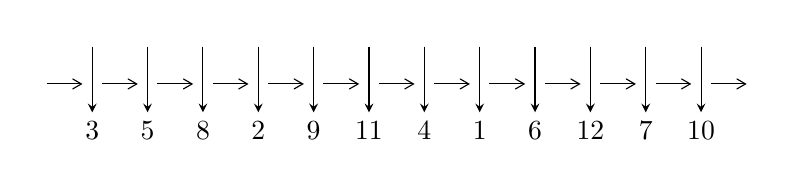
\begin{tikzpicture}[x=20pt, y=17pt]
	% nodes
	\node (C0) at (0, 0) {};
	\node (C1) at (1, 0) {};
	\node (C1U) at (1, +1) {};
	\node (C1D) at (1, -1) {3};

	\node (C2) at (2, 0) {};
	\node (C2U) at (2, +1) {};
	\node (C2D) at (2, -1) {5};

	\node (C3) at (3, 0) {};
	\node (C3U) at (3, +1) {};
	\node (C3D) at (3, -1) {8};

	\node (C4) at (4, 0) {};
	\node (C4U) at (4, +1) {};
	\node (C4D) at (4, -1) {2};

	\node (C5) at (5, 0) {};
	\node (C5U) at (5, +1) {};
	\node (C5D) at (5, -1) {9};

	\node (C6) at (6, 0) {};
	\node (C6U) at (6, +1) {};
	\node (C6D) at (6, -1) {11};

	\node (C7) at (7, 0) {};
	\node (C7U) at (7, +1) {};
	\node (C7D) at (7, -1) {4};

	\node (C8) at (8, 0) {};
	\node (C8U) at (8, +1) {};
	\node (C8D) at (8, -1) {1};

	\node (C9) at (9, 0) {};
	\node (C9U) at (9, +1) {};
	\node (C9D) at (9, -1) {6};

	\node (C10) at (10, 0) {};
	\node (C10U) at (10, +1) {};
	\node (C10D) at (10, -1) {12};

	\node (C11) at (11, 0) {};
	\node (C11U) at (11, +1) {};
	\node (C11D) at (11, -1) {7};

	\node (C12) at (12, 0) {};
	\node (C12U) at (12, +1) {};
	\node (C12D) at (12, -1) {10};
	\node (C13) at (13, 0) {};

	% arrows
	\draw[->,>={angle 60}]
	(C0) edge (C1) (C1) edge (C2) (C2) edge (C3) (C3) edge (C4) (C4) edge (C5) (C5) edge (C6) (C6) edge (C7) (C7) edge (C8) (C8) edge (C9) (C9) edge (C10) (C10) edge (C11) (C11) edge (C12) (C12) edge (C13) ;	\draw[->,>=stealth]
	(C1U) edge (C1D) (C2U) edge (C2D) (C3U) edge (C3D) (C4U) edge (C4D) (C5U) edge (C5D) (C6U) edge (C6D) (C7U) edge (C7D) (C8U) edge (C8D) (C9U) edge (C9D) (C10U) edge (C10D) (C11U) edge (C11D) (C12U) edge (C12D) ;
	\end{tikzpicture} \\
\hhline{~~} \\& 
\textbf{Solving Sequence} \\ \cline{2-2} 
 &
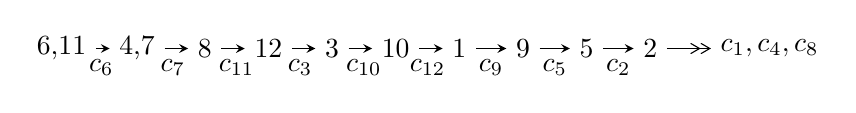
\begin{tikzpicture}[x=23pt, y=7pt]
	% node
	\node (A0) at (-1/8, 0) {6,11};
	\node (A1) at (17/16, 0) {4,7};
	\node (A2) at (17/8, 0) {8};
	\node (A3) at (25/8, 0) {12};
	\node (A4) at (33/8, 0) {3};
	\node (A5) at (41/8, 0) {10};
	\node (A6) at (49/8, 0) {1};
	\node (A7) at (57/8, 0) {9};
	\node (A8) at (65/8, 0) {5};
	\node (A9) at (73/8, 0) {2};
	\node (C1) at (1/2, -1) {$c_{6}$};
	\node (C2) at (13/8, -1) {$c_{7}$};
	\node (C3) at (21/8, -1) {$c_{11}$};
	\node (C4) at (29/8, -1) {$c_{3}$};
	\node (C5) at (37/8, -1) {$c_{10}$};
	\node (C6) at (45/8, -1) {$c_{12}$};
	\node (C7) at (53/8, -1) {$c_{9}$};
	\node (C8) at (61/8, -1) {$c_{5}$};
	\node (C9) at (69/8, -1) {$c_{2}$};
	\node (A10) at (11, 0) {$c_{1},c_{4},c_{8}$};

	% edge
	\draw[->,>=stealth]	
	(A0) edge (A1) (A1) edge (A2) (A2) edge (A3) (A3) edge (A4) (A4) edge (A5) (A5) edge (A6) (A6) edge (A7) (A7) edge (A8) (A8) edge (A9) ;
	\draw[->>,>={angle 60}]	
	(A9) edge (A10);
\end{tikzpicture} \\ 

\end{tabular} \\

\footnotetext{
The image of knot diagram is generated by the software ``\textbf{Draw programme}" developed by Andrew Bartholomew(\url{http://www.layer8.co.uk/maths/draw/index.htm\#Running-draw}), where we modified some parts for our purpose(\url{https://github.com/CATsTAILs/LinksPainter}).
}\phantom \\ \newline 
\centering \textbf{Ideals for irreducible components\footnotemark of $X_{\text{par}}$} 
 
\begin{align*}
I^u_{1}&=\langle 
u^{102}+u^{101}+\cdots+b-1,\;- u^{99}+16 u^{97}+\cdots+a+2 u,\;u^{103}+2 u^{102}+\cdots+6 u^2-1\rangle \\
I^u_{2}&=\langle 
u^7- u^5+2 u^3+b- u+1,\;u^7- u^5+u^4+2 u^3- u^2+a+2,\;u^8- u^7- u^6+2 u^5+u^4-2 u^3+2 u-1\rangle \\
\\
\end{align*}
\raggedright * 2 irreducible components of $\dim_{\mathbb{C}}=0$, with total 111 representations.\\
\footnotetext{All coefficients of polynomials are rational numbers. But the coefficients are sometimes approximated in decimal forms when there is not enough margin.}
\newpage
\renewcommand{\arraystretch}{1}
\centering \section*{I. $I^u_{1}= \langle u^{102}+u^{101}+\cdots+b-1,\;- u^{99}+16 u^{97}+\cdots+a+2 u,\;u^{103}+2 u^{102}+\cdots+6 u^2-1 \rangle$}
\flushleft \textbf{(i) Arc colorings}\\
\begin{tabular}{m{7pt} m{180pt} m{7pt} m{180pt} }
\flushright $a_{6}=$&$\begin{pmatrix}1\\0\end{pmatrix}$ \\
\flushright $a_{11}=$&$\begin{pmatrix}0\\u\end{pmatrix}$ \\
\flushright $a_{4}=$&$\begin{pmatrix}u^{99}-16 u^{97}+\cdots-3 u^2-2 u\\- u^{102}- u^{101}+\cdots+u+1\end{pmatrix}$ \\
\flushright $a_{7}=$&$\begin{pmatrix}1\\u^2\end{pmatrix}$ \\
\flushright $a_{8}=$&$\begin{pmatrix}- u^{17}+2 u^{15}-5 u^{13}+6 u^{11}-7 u^9+6 u^7-2 u^5+2 u^3+u\\- u^{19}+3 u^{17}-8 u^{15}+13 u^{13}-17 u^{11}+17 u^9-12 u^7+8 u^5-3 u^3+u\end{pmatrix}$ \\
\flushright $a_{12}=$&$\begin{pmatrix}- u\\- u^3+u\end{pmatrix}$ \\
\flushright $a_{3}=$&$\begin{pmatrix}-2 u^{102}-2 u^{101}+\cdots-3 u+1\\- u^{102}- u^{101}+\cdots-4 u^2+1\end{pmatrix}$ \\
\flushright $a_{10}=$&$\begin{pmatrix}u^3\\u^5- u^3+u\end{pmatrix}$ \\
\flushright $a_{1}=$&$\begin{pmatrix}- u^5- u\\- u^7+u^5-2 u^3+u\end{pmatrix}$ \\
\flushright $a_{9}=$&$\begin{pmatrix}u^5+u\\u^5- u^3+u\end{pmatrix}$ \\
\flushright $a_{5}=$&$\begin{pmatrix}- u^{10}+u^8-2 u^6+u^4- u^2+1\\- u^{10}+2 u^8-3 u^6+2 u^4- u^2\end{pmatrix}$ \\
\flushright $a_{2}=$&$\begin{pmatrix}- u^{102}- u^{101}+\cdots-2 u+1\\- u^{102}- u^{101}+\cdots+u+1\end{pmatrix}$\\&\end{tabular}
\flushleft \textbf{(ii) Obstruction class $= -1$}\\~\\
\flushleft \textbf{(iii) Cusp Shapes $= 11 u^{102}+10 u^{101}+\cdots-4 u-21$}\\~\\
\newpage\renewcommand{\arraystretch}{1}
\flushleft \textbf{(iv) u-Polynomials at the component}\newline \\
\begin{tabular}{m{50pt}|m{274pt}}
Crossings & \hspace{64pt}u-Polynomials at each crossing \\
\hline $$\begin{aligned}c_{1}\end{aligned}$$&$\begin{aligned}
&u^{103}+49 u^{102}+\cdots+72 u+1
\end{aligned}$\\
\hline $$\begin{aligned}c_{2},c_{4}\end{aligned}$$&$\begin{aligned}
&u^{103}-9 u^{102}+\cdots-2 u+1
\end{aligned}$\\
\hline $$\begin{aligned}c_{3},c_{7}\end{aligned}$$&$\begin{aligned}
&u^{103}+u^{102}+\cdots+896 u+256
\end{aligned}$\\
\hline $$\begin{aligned}c_{5},c_{9}\end{aligned}$$&$\begin{aligned}
&u^{103}+2 u^{102}+\cdots+126 u+9
\end{aligned}$\\
\hline $$\begin{aligned}c_{6},c_{11}\end{aligned}$$&$\begin{aligned}
&u^{103}-2 u^{102}+\cdots-6 u^2+1
\end{aligned}$\\
\hline $$\begin{aligned}c_{8}\end{aligned}$$&$\begin{aligned}
&u^{103}-8 u^{102}+\cdots+326018 u+52865
\end{aligned}$\\
\hline $$\begin{aligned}c_{10},c_{12}\end{aligned}$$&$\begin{aligned}
&u^{103}+36 u^{102}+\cdots+12 u+1
\end{aligned}$\\
\hline
\end{tabular}\\~\\
\newpage\renewcommand{\arraystretch}{1}
\flushleft \textbf{(v) Riley Polynomials at the component}\newline \\
\begin{tabular}{m{50pt}|m{274pt}}
Crossings & \hspace{64pt}Riley Polynomials at each crossing \\
\hline $$\begin{aligned}c_{1}\end{aligned}$$&$\begin{aligned}
&y^{103}+19 y^{102}+\cdots+1672 y-1
\end{aligned}$\\
\hline $$\begin{aligned}c_{2},c_{4}\end{aligned}$$&$\begin{aligned}
&y^{103}-49 y^{102}+\cdots+72 y-1
\end{aligned}$\\
\hline $$\begin{aligned}c_{3},c_{7}\end{aligned}$$&$\begin{aligned}
&y^{103}+51 y^{102}+\cdots-1130496 y-65536
\end{aligned}$\\
\hline $$\begin{aligned}c_{5},c_{9}\end{aligned}$$&$\begin{aligned}
&y^{103}-68 y^{102}+\cdots-22536 y-81
\end{aligned}$\\
\hline $$\begin{aligned}c_{6},c_{11}\end{aligned}$$&$\begin{aligned}
&y^{103}-36 y^{102}+\cdots+12 y-1
\end{aligned}$\\
\hline $$\begin{aligned}c_{8}\end{aligned}$$&$\begin{aligned}
&y^{103}+16 y^{102}+\cdots-53970185116 y-2794708225
\end{aligned}$\\
\hline $$\begin{aligned}c_{10},c_{12}\end{aligned}$$&$\begin{aligned}
&y^{103}+64 y^{102}+\cdots-68 y-1
\end{aligned}$\\
\hline
\end{tabular}\\~\\
\newpage\flushleft \textbf{(vi) Complex Volumes and Cusp Shapes}
$$\begin{array}{c|c|c}  
\text{Solutions to }I^u_{1}& \I (\text{vol} + \sqrt{-1}CS) & \text{Cusp shape}\\
 \hline 
\begin{aligned}
u &= -0.912335 + 0.408500 I \\
a &= \phantom{-}2.31902 - 0.54728 I \\
b &= \phantom{-}0.584528 - 0.968145 I\end{aligned}
 & \phantom{-}0.08009 + 7.90391 I & \phantom{-0.000000 } 0 \\ \hline\begin{aligned}
u &= -0.912335 - 0.408500 I \\
a &= \phantom{-}2.31902 + 0.54728 I \\
b &= \phantom{-}0.584528 + 0.968145 I\end{aligned}
 & \phantom{-}0.08009 - 7.90391 I & \phantom{-0.000000 } 0 \\ \hline\begin{aligned}
u &= \phantom{-}0.616846 + 0.780917 I \\
a &= \phantom{-}0.639980 + 0.490478 I \\
b &= -1.65356 + 0.05660 I\end{aligned}
 & -0.99710 + 5.42375 I & \phantom{-0.000000 } 0 \\ \hline\begin{aligned}
u &= \phantom{-}0.616846 - 0.780917 I \\
a &= \phantom{-}0.639980 - 0.490478 I \\
b &= -1.65356 - 0.05660 I\end{aligned}
 & -0.99710 - 5.42375 I & \phantom{-0.000000 } 0 \\ \hline\begin{aligned}
u &= -0.881449 + 0.484517 I \\
a &= -1.60696 + 0.38647 I \\
b &= -0.254925 + 0.557993 I\end{aligned}
 & \phantom{-}1.89796 + 2.95652 I & \phantom{-0.000000 } 0 \\ \hline\begin{aligned}
u &= -0.881449 - 0.484517 I \\
a &= -1.60696 - 0.38647 I \\
b &= -0.254925 - 0.557993 I\end{aligned}
 & \phantom{-}1.89796 - 2.95652 I & \phantom{-0.000000 } 0 \\ \hline\begin{aligned}
u &= \phantom{-}1.005320 + 0.087510 I \\
a &= \phantom{-}0.54041 + 1.59055 I \\
b &= \phantom{-}0.289073 + 0.524898 I\end{aligned}
 & -0.23823 - 2.28486 I & \phantom{-0.000000 } 0 \\ \hline\begin{aligned}
u &= \phantom{-}1.005320 - 0.087510 I \\
a &= \phantom{-}0.54041 - 1.59055 I \\
b &= \phantom{-}0.289073 - 0.524898 I\end{aligned}
 & -0.23823 + 2.28486 I & \phantom{-0.000000 } 0 \\ \hline\begin{aligned}
u &= -0.624209 + 0.794738 I \\
a &= -1.097790 + 0.679494 I \\
b &= \phantom{-}1.43840 + 2.14786 I\end{aligned}
 & \phantom{-}3.77337 - 6.03756 I & \phantom{-0.000000 } 0 \\ \hline\begin{aligned}
u &= -0.624209 - 0.794738 I \\
a &= -1.097790 - 0.679494 I \\
b &= \phantom{-}1.43840 - 2.14786 I\end{aligned}
 & \phantom{-}3.77337 + 6.03756 I & \phantom{-0.000000 } 0\\
 \hline 
 \end{array}$$\newpage$$\begin{array}{c|c|c}  
\text{Solutions to }I^u_{1}& \I (\text{vol} + \sqrt{-1}CS) & \text{Cusp shape}\\
 \hline 
\begin{aligned}
u &= -0.613526 + 0.803225 I \\
a &= \phantom{-}1.31576 - 0.53967 I \\
b &= -1.56697 - 2.36415 I\end{aligned}
 & \phantom{-}1.44101 - 11.65940 I & \phantom{-0.000000 } 0 \\ \hline\begin{aligned}
u &= -0.613526 - 0.803225 I \\
a &= \phantom{-}1.31576 + 0.53967 I \\
b &= -1.56697 + 2.36415 I\end{aligned}
 & \phantom{-}1.44101 + 11.65940 I & \phantom{-0.000000 } 0 \\ \hline\begin{aligned}
u &= -0.614579 + 0.767089 I \\
a &= \phantom{-}1.15511 - 1.33576 I \\
b &= -1.84696 - 1.71453 I\end{aligned}
 & -1.91217 - 2.88103 I & \phantom{-0.000000 } 0 \\ \hline\begin{aligned}
u &= -0.614579 - 0.767089 I \\
a &= \phantom{-}1.15511 + 1.33576 I \\
b &= -1.84696 + 1.71453 I\end{aligned}
 & -1.91217 + 2.88103 I & \phantom{-0.000000 } 0 \\ \hline\begin{aligned}
u &= \phantom{-}0.631063 + 0.747905 I \\
a &= -0.656987 - 0.310998 I \\
b &= \phantom{-}1.314400 - 0.477130 I\end{aligned}
 & \phantom{-}0.307513 + 1.061580 I & \phantom{-0.000000 } 0 \\ \hline\begin{aligned}
u &= \phantom{-}0.631063 - 0.747905 I \\
a &= -0.656987 + 0.310998 I \\
b &= \phantom{-}1.314400 + 0.477130 I\end{aligned}
 & \phantom{-}0.307513 - 1.061580 I & \phantom{-0.000000 } 0 \\ \hline\begin{aligned}
u &= -0.672704 + 0.770186 I \\
a &= -0.233235 + 0.783530 I \\
b &= \phantom{-}0.75052 + 1.40903 I\end{aligned}
 & \phantom{-}5.58134 - 2.28100 I & \phantom{-0.000000 } 0 \\ \hline\begin{aligned}
u &= -0.672704 - 0.770186 I \\
a &= -0.233235 - 0.783530 I \\
b &= \phantom{-}0.75052 - 1.40903 I\end{aligned}
 & \phantom{-}5.58134 + 2.28100 I & \phantom{-0.000000 } 0 \\ \hline\begin{aligned}
u &= -0.702746 + 0.759112 I \\
a &= -0.085346 - 0.728100 I \\
b &= -0.403150 - 1.083490 I\end{aligned}
 & \phantom{-}4.66987 + 3.22738 I & \phantom{-0.000000 } 0 \\ \hline\begin{aligned}
u &= -0.702746 - 0.759112 I \\
a &= -0.085346 + 0.728100 I \\
b &= -0.403150 + 1.083490 I\end{aligned}
 & \phantom{-}4.66987 - 3.22738 I & \phantom{-0.000000 } 0\\
 \hline 
 \end{array}$$\newpage$$\begin{array}{c|c|c}  
\text{Solutions to }I^u_{1}& \I (\text{vol} + \sqrt{-1}CS) & \text{Cusp shape}\\
 \hline 
\begin{aligned}
u &= \phantom{-}0.559939 + 0.767741 I \\
a &= \phantom{-}0.186132 + 0.629586 I \\
b &= -0.911639 - 0.783862 I\end{aligned}
 & -2.37667 - 0.08774 I & \phantom{-0.000000 } 0 \\ \hline\begin{aligned}
u &= \phantom{-}0.559939 - 0.767741 I \\
a &= \phantom{-}0.186132 - 0.629586 I \\
b &= -0.911639 + 0.783862 I\end{aligned}
 & -2.37667 + 0.08774 I & \phantom{-0.000000 } 0 \\ \hline\begin{aligned}
u &= \phantom{-}0.934664 + 0.166620 I \\
a &= \phantom{-}0.25189 - 1.89766 I \\
b &= \phantom{-}0.409310 - 0.451135 I\end{aligned}
 & -1.07874 + 2.57674 I & \phantom{-0.000000 } 0 \\ \hline\begin{aligned}
u &= \phantom{-}0.934664 - 0.166620 I \\
a &= \phantom{-}0.25189 + 1.89766 I \\
b &= \phantom{-}0.409310 + 0.451135 I\end{aligned}
 & -1.07874 - 2.57674 I & \phantom{-0.000000 } 0 \\ \hline\begin{aligned}
u &= -0.853017 + 0.633169 I \\
a &= -0.533821 + 0.009715 I \\
b &= -0.1065160 + 0.0398102 I\end{aligned}
 & \phantom{-}1.77380 + 2.47815 I & \phantom{-0.000000 } 0 \\ \hline\begin{aligned}
u &= -0.853017 - 0.633169 I \\
a &= -0.533821 - 0.009715 I \\
b &= -0.1065160 - 0.0398102 I\end{aligned}
 & \phantom{-}1.77380 - 2.47815 I & \phantom{-0.000000 } 0 \\ \hline\begin{aligned}
u &= -1.067130 + 0.027007 I \\
a &= \phantom{-}2.20309 + 0.64129 I \\
b &= \phantom{-}1.68580 + 0.39940 I\end{aligned}
 & -5.25977 + 0.42586 I & \phantom{-0.000000 } 0 \\ \hline\begin{aligned}
u &= -1.067130 - 0.027007 I \\
a &= \phantom{-}2.20309 - 0.64129 I \\
b &= \phantom{-}1.68580 - 0.39940 I\end{aligned}
 & -5.25977 - 0.42586 I & \phantom{-0.000000 } 0 \\ \hline\begin{aligned}
u &= \phantom{-}1.085050 + 0.040939 I \\
a &= -2.07495 - 0.29647 I \\
b &= -1.99607 + 0.35332 I\end{aligned}
 & -7.69423 - 2.11350 I & \phantom{-0.000000 } 0 \\ \hline\begin{aligned}
u &= \phantom{-}1.085050 - 0.040939 I \\
a &= -2.07495 + 0.29647 I \\
b &= -1.99607 - 0.35332 I\end{aligned}
 & -7.69423 + 2.11350 I & \phantom{-0.000000 } 0\\
 \hline 
 \end{array}$$\newpage$$\begin{array}{c|c|c}  
\text{Solutions to }I^u_{1}& \I (\text{vol} + \sqrt{-1}CS) & \text{Cusp shape}\\
 \hline 
\begin{aligned}
u &= -1.089270 + 0.053148 I \\
a &= -2.37201 - 1.44590 I \\
b &= -1.97109 - 0.94572 I\end{aligned}
 & -6.91666 + 4.67542 I & \phantom{-0.000000 } 0 \\ \hline\begin{aligned}
u &= -1.089270 - 0.053148 I \\
a &= -2.37201 + 1.44590 I \\
b &= -1.97109 + 0.94572 I\end{aligned}
 & -6.91666 - 4.67542 I & \phantom{-0.000000 } 0 \\ \hline\begin{aligned}
u &= \phantom{-}1.091240 + 0.069455 I \\
a &= \phantom{-}2.22714 + 1.29507 I \\
b &= \phantom{-}1.93126 + 0.69834 I\end{aligned}
 & -2.30120 - 5.35216 I & \phantom{-0.000000 } 0 \\ \hline\begin{aligned}
u &= \phantom{-}1.091240 - 0.069455 I \\
a &= \phantom{-}2.22714 - 1.29507 I \\
b &= \phantom{-}1.93126 - 0.69834 I\end{aligned}
 & -2.30120 + 5.35216 I & \phantom{-0.000000 } 0 \\ \hline\begin{aligned}
u &= \phantom{-}0.606096 + 0.662511 I \\
a &= -0.798963 + 0.126546 I \\
b &= \phantom{-}0.649948 - 0.932632 I\end{aligned}
 & -0.302081 + 0.540644 I & \phantom{-0.000000 } 0 \\ \hline\begin{aligned}
u &= \phantom{-}0.606096 - 0.662511 I \\
a &= -0.798963 - 0.126546 I \\
b &= \phantom{-}0.649948 + 0.932632 I\end{aligned}
 & -0.302081 - 0.540644 I & \phantom{-0.000000 } 0 \\ \hline\begin{aligned}
u &= \phantom{-}0.511993 + 0.732368 I \\
a &= \phantom{-}0.343675 - 0.709475 I \\
b &= \phantom{-}0.044302 + 1.277450 I\end{aligned}
 & -2.69016 + 2.77408 I & \phantom{-0.000000 } 0 \\ \hline\begin{aligned}
u &= \phantom{-}0.511993 - 0.732368 I \\
a &= \phantom{-}0.343675 + 0.709475 I \\
b &= \phantom{-}0.044302 - 1.277450 I\end{aligned}
 & -2.69016 - 2.77408 I & \phantom{-0.000000 } 0 \\ \hline\begin{aligned}
u &= \phantom{-}1.106320 + 0.068441 I \\
a &= -2.68986 - 1.37616 I \\
b &= -2.38599 - 0.90186 I\end{aligned}
 & -4.70352 - 10.84140 I & \phantom{-0.000000 } 0 \\ \hline\begin{aligned}
u &= \phantom{-}1.106320 - 0.068441 I \\
a &= -2.68986 + 1.37616 I \\
b &= -2.38599 + 0.90186 I\end{aligned}
 & -4.70352 + 10.84140 I & \phantom{-0.000000 } 0\\
 \hline 
 \end{array}$$\newpage$$\begin{array}{c|c|c}  
\text{Solutions to }I^u_{1}& \I (\text{vol} + \sqrt{-1}CS) & \text{Cusp shape}\\
 \hline 
\begin{aligned}
u &= -0.842412 + 0.726529 I \\
a &= -0.178651 - 0.729133 I \\
b &= \phantom{-}0.0579763 - 0.1150040 I\end{aligned}
 & \phantom{-}3.07344 + 0.63735 I & \phantom{-0.000000 } 0 \\ \hline\begin{aligned}
u &= -0.842412 - 0.726529 I \\
a &= -0.178651 + 0.729133 I \\
b &= \phantom{-}0.0579763 + 0.1150040 I\end{aligned}
 & \phantom{-}3.07344 - 0.63735 I & \phantom{-0.000000 } 0 \\ \hline\begin{aligned}
u &= -1.116010 + 0.016772 I \\
a &= -0.84995 - 1.85919 I \\
b &= -0.75181 - 1.51606 I\end{aligned}
 & -8.11122 - 1.30695 I & \phantom{-0.000000 } 0 \\ \hline\begin{aligned}
u &= -1.116010 - 0.016772 I \\
a &= -0.84995 + 1.85919 I \\
b &= -0.75181 + 1.51606 I\end{aligned}
 & -8.11122 + 1.30695 I & \phantom{-0.000000 } 0 \\ \hline\begin{aligned}
u &= \phantom{-}0.859325 + 0.712441 I \\
a &= \phantom{-}0.75900 - 2.33832 I \\
b &= \phantom{-}3.00650 - 0.45544 I\end{aligned}
 & \phantom{-}1.60340 - 2.72171 I & \phantom{-0.000000 } 0 \\ \hline\begin{aligned}
u &= \phantom{-}0.859325 - 0.712441 I \\
a &= \phantom{-}0.75900 + 2.33832 I \\
b &= \phantom{-}3.00650 + 0.45544 I\end{aligned}
 & \phantom{-}1.60340 + 2.72171 I & \phantom{-0.000000 } 0 \\ \hline\begin{aligned}
u &= \phantom{-}0.823392 + 0.756871 I \\
a &= \phantom{-}0.218483 - 0.973336 I \\
b &= \phantom{-}1.78019 - 1.08683 I\end{aligned}
 & \phantom{-}6.43694 + 4.87550 I & \phantom{-0.000000 } 0 \\ \hline\begin{aligned}
u &= \phantom{-}0.823392 - 0.756871 I \\
a &= \phantom{-}0.218483 + 0.973336 I \\
b &= \phantom{-}1.78019 + 1.08683 I\end{aligned}
 & \phantom{-}6.43694 - 4.87550 I & \phantom{-0.000000 } 0 \\ \hline\begin{aligned}
u &= \phantom{-}0.770289 + 0.411262 I \\
a &= \phantom{-}1.47793 - 0.96752 I \\
b &= \phantom{-}0.440891 + 0.958529 I\end{aligned}
 & -2.10537 - 2.84140 I & \phantom{-0.000000 } 0 \\ \hline\begin{aligned}
u &= \phantom{-}0.770289 - 0.411262 I \\
a &= \phantom{-}1.47793 + 0.96752 I \\
b &= \phantom{-}0.440891 - 0.958529 I\end{aligned}
 & -2.10537 + 2.84140 I & \phantom{-0.000000 } 0\\
 \hline 
 \end{array}$$\newpage$$\begin{array}{c|c|c}  
\text{Solutions to }I^u_{1}& \I (\text{vol} + \sqrt{-1}CS) & \text{Cusp shape}\\
 \hline 
\begin{aligned}
u &= \phantom{-}0.841098 + 0.751122 I \\
a &= -0.506788 + 1.209090 I \\
b &= -1.90230 + 0.81017 I\end{aligned}
 & \phantom{-}8.10016 - 0.78832 I & \phantom{-0.000000 } 0 \\ \hline\begin{aligned}
u &= \phantom{-}0.841098 - 0.751122 I \\
a &= -0.506788 - 1.209090 I \\
b &= -1.90230 - 0.81017 I\end{aligned}
 & \phantom{-}8.10016 + 0.78832 I & \phantom{-0.000000 } 0 \\ \hline\begin{aligned}
u &= -0.876875 + 0.722197 I \\
a &= -0.091761 + 0.802743 I \\
b &= -0.0013840 + 0.0733994 I\end{aligned}
 & \phantom{-}2.96916 + 4.87835 I & \phantom{-0.000000 } 0 \\ \hline\begin{aligned}
u &= -0.876875 - 0.722197 I \\
a &= -0.091761 - 0.802743 I \\
b &= -0.0013840 - 0.0733994 I\end{aligned}
 & \phantom{-}2.96916 - 4.87835 I & \phantom{-0.000000 } 0 \\ \hline\begin{aligned}
u &= \phantom{-}0.885183 + 0.741783 I \\
a &= -1.39537 + 1.55461 I \\
b &= -2.03510 - 0.19569 I\end{aligned}
 & \phantom{-}7.96620 - 4.86085 I & \phantom{-0.000000 } 0 \\ \hline\begin{aligned}
u &= \phantom{-}0.885183 - 0.741783 I \\
a &= -1.39537 - 1.55461 I \\
b &= -2.03510 + 0.19569 I\end{aligned}
 & \phantom{-}7.96620 + 4.86085 I & \phantom{-0.000000 } 0 \\ \hline\begin{aligned}
u &= \phantom{-}0.901166 + 0.740058 I \\
a &= \phantom{-}1.66978 - 1.57705 I \\
b &= \phantom{-}1.97824 + 0.55475 I\end{aligned}
 & \phantom{-}6.20092 - 10.53630 I & \phantom{-0.000000 } 0 \\ \hline\begin{aligned}
u &= \phantom{-}0.901166 - 0.740058 I \\
a &= \phantom{-}1.66978 + 1.57705 I \\
b &= \phantom{-}1.97824 - 0.55475 I\end{aligned}
 & \phantom{-}6.20092 + 10.53630 I & \phantom{-0.000000 } 0 \\ \hline\begin{aligned}
u &= -1.005990 + 0.592232 I \\
a &= \phantom{-}0.167955 + 1.051150 I \\
b &= \phantom{-}0.878165 - 0.601426 I\end{aligned}
 & \phantom{-}0.848394 + 1.048560 I & \phantom{-0.000000 } 0 \\ \hline\begin{aligned}
u &= -1.005990 - 0.592232 I \\
a &= \phantom{-}0.167955 - 1.051150 I \\
b &= \phantom{-}0.878165 + 0.601426 I\end{aligned}
 & \phantom{-}0.848394 - 1.048560 I & \phantom{-0.000000 } 0\\
 \hline 
 \end{array}$$\newpage$$\begin{array}{c|c|c}  
\text{Solutions to }I^u_{1}& \I (\text{vol} + \sqrt{-1}CS) & \text{Cusp shape}\\
 \hline 
\begin{aligned}
u &= \phantom{-}1.011120 + 0.612755 I \\
a &= -2.26014 + 0.37543 I \\
b &= -0.99132 - 2.03559 I\end{aligned}
 & -3.51458 - 1.68605 I & \phantom{-0.000000 } 0 \\ \hline\begin{aligned}
u &= \phantom{-}1.011120 - 0.612755 I \\
a &= -2.26014 - 0.37543 I \\
b &= -0.99132 + 2.03559 I\end{aligned}
 & -3.51458 + 1.68605 I & \phantom{-0.000000 } 0 \\ \hline\begin{aligned}
u &= -1.026270 + 0.590666 I \\
a &= -0.53736 - 1.42442 I \\
b &= -1.44389 + 0.79586 I\end{aligned}
 & -1.50754 - 4.20851 I & \phantom{-0.000000 } 0 \\ \hline\begin{aligned}
u &= -1.026270 - 0.590666 I \\
a &= -0.53736 + 1.42442 I \\
b &= -1.44389 - 0.79586 I\end{aligned}
 & -1.50754 + 4.20851 I & \phantom{-0.000000 } 0 \\ \hline\begin{aligned}
u &= -1.012950 + 0.625812 I \\
a &= -0.700288 - 0.186711 I \\
b &= -0.19292 + 1.59502 I\end{aligned}
 & -4.11619 + 4.19240 I & \phantom{-0.000000 } 0 \\ \hline\begin{aligned}
u &= -1.012950 - 0.625812 I \\
a &= -0.700288 + 0.186711 I \\
b &= -0.19292 - 1.59502 I\end{aligned}
 & -4.11619 - 4.19240 I & \phantom{-0.000000 } 0 \\ \hline\begin{aligned}
u &= \phantom{-}1.007840 + 0.644172 I \\
a &= \phantom{-}1.61422 - 0.67239 I \\
b &= \phantom{-}1.06573 + 1.37400 I\end{aligned}
 & -1.46823 - 5.66596 I & \phantom{-0.000000 } 0 \\ \hline\begin{aligned}
u &= \phantom{-}1.007840 - 0.644172 I \\
a &= \phantom{-}1.61422 + 0.67239 I \\
b &= \phantom{-}1.06573 - 1.37400 I\end{aligned}
 & -1.46823 + 5.66596 I & \phantom{-0.000000 } 0 \\ \hline\begin{aligned}
u &= -0.516513 + 0.614538 I \\
a &= \phantom{-}1.61419 + 1.13685 I \\
b &= \phantom{-}0.114440 - 0.378217 I\end{aligned}
 & -2.79751 + 0.75492 I & -13.18461 - 4.17377 I \\ \hline\begin{aligned}
u &= -0.516513 - 0.614538 I \\
a &= \phantom{-}1.61419 - 1.13685 I \\
b &= \phantom{-}0.114440 + 0.378217 I\end{aligned}
 & -2.79751 - 0.75492 I & -13.18461 + 4.17377 I\\
 \hline 
 \end{array}$$\newpage$$\begin{array}{c|c|c}  
\text{Solutions to }I^u_{1}& \I (\text{vol} + \sqrt{-1}CS) & \text{Cusp shape}\\
 \hline 
\begin{aligned}
u &= -0.984760 + 0.696068 I \\
a &= -1.354280 + 0.257551 I \\
b &= -0.630888 + 0.742129 I\end{aligned}
 & \phantom{-}3.81659 + 2.30298 I & \phantom{-0.000000 } 0 \\ \hline\begin{aligned}
u &= -0.984760 - 0.696068 I \\
a &= -1.354280 - 0.257551 I \\
b &= -0.630888 - 0.742129 I\end{aligned}
 & \phantom{-}3.81659 - 2.30298 I & \phantom{-0.000000 } 0 \\ \hline\begin{aligned}
u &= -0.392378 + 0.674009 I \\
a &= \phantom{-}1.55257 + 0.40077 I \\
b &= -0.903906 + 0.236031 I\end{aligned}
 & \phantom{-}0.18178 + 8.98054 I & -11.00021 - 7.46838 I \\ \hline\begin{aligned}
u &= -0.392378 - 0.674009 I \\
a &= \phantom{-}1.55257 - 0.40077 I \\
b &= -0.903906 - 0.236031 I\end{aligned}
 & \phantom{-}0.18178 - 8.98054 I & -11.00021 + 7.46838 I \\ \hline\begin{aligned}
u &= -1.004500 + 0.695052 I \\
a &= \phantom{-}1.79376 + 0.08698 I \\
b &= \phantom{-}1.12781 - 1.16810 I\end{aligned}
 & \phantom{-}4.58233 + 7.83910 I & \phantom{-0.000000 } 0 \\ \hline\begin{aligned}
u &= -1.004500 - 0.695052 I \\
a &= \phantom{-}1.79376 - 0.08698 I \\
b &= \phantom{-}1.12781 + 1.16810 I\end{aligned}
 & \phantom{-}4.58233 - 7.83910 I & \phantom{-0.000000 } 0 \\ \hline\begin{aligned}
u &= \phantom{-}1.042120 + 0.637671 I \\
a &= -1.61249 - 0.63861 I \\
b &= \phantom{-}0.17740 - 1.77018 I\end{aligned}
 & -4.20496 - 7.99344 I & \phantom{-0.000000 } 0 \\ \hline\begin{aligned}
u &= \phantom{-}1.042120 - 0.637671 I \\
a &= -1.61249 + 0.63861 I \\
b &= \phantom{-}0.17740 + 1.77018 I\end{aligned}
 & -4.20496 + 7.99344 I & \phantom{-0.000000 } 0 \\ \hline\begin{aligned}
u &= \phantom{-}1.018180 + 0.675918 I \\
a &= \phantom{-}0.96849 - 1.49648 I \\
b &= \phantom{-}1.68010 + 0.59427 I\end{aligned}
 & -0.84382 - 6.49823 I & \phantom{-0.000000 } 0 \\ \hline\begin{aligned}
u &= \phantom{-}1.018180 - 0.675918 I \\
a &= \phantom{-}0.96849 + 1.49648 I \\
b &= \phantom{-}1.68010 - 0.59427 I\end{aligned}
 & -0.84382 + 6.49823 I & \phantom{-0.000000 } 0\\
 \hline 
 \end{array}$$\newpage$$\begin{array}{c|c|c}  
\text{Solutions to }I^u_{1}& \I (\text{vol} + \sqrt{-1}CS) & \text{Cusp shape}\\
 \hline 
\begin{aligned}
u &= -1.028310 + 0.678590 I \\
a &= -2.41921 - 1.22556 I \\
b &= -2.79352 + 1.71272 I\end{aligned}
 & -3.14095 + 8.37153 I & \phantom{-0.000000 } 0 \\ \hline\begin{aligned}
u &= -1.028310 - 0.678590 I \\
a &= -2.41921 + 1.22556 I \\
b &= -2.79352 - 1.71272 I\end{aligned}
 & -3.14095 - 8.37153 I & \phantom{-0.000000 } 0 \\ \hline\begin{aligned}
u &= \phantom{-}1.044270 + 0.661570 I \\
a &= \phantom{-}0.50721 + 1.38026 I \\
b &= -1.25248 + 0.85970 I\end{aligned}
 & -3.79812 - 5.32874 I & \phantom{-0.000000 } 0 \\ \hline\begin{aligned}
u &= \phantom{-}1.044270 - 0.661570 I \\
a &= \phantom{-}0.50721 - 1.38026 I \\
b &= -1.25248 - 0.85970 I\end{aligned}
 & -3.79812 + 5.32874 I & \phantom{-0.000000 } 0 \\ \hline\begin{aligned}
u &= \phantom{-}1.031540 + 0.683934 I \\
a &= -0.62182 + 1.93629 I \\
b &= -2.05487 - 0.18548 I\end{aligned}
 & -2.23392 - 10.96790 I & \phantom{-0.000000 } 0 \\ \hline\begin{aligned}
u &= \phantom{-}1.031540 - 0.683934 I \\
a &= -0.62182 - 1.93629 I \\
b &= -2.05487 + 0.18548 I\end{aligned}
 & -2.23392 + 10.96790 I & \phantom{-0.000000 } 0 \\ \hline\begin{aligned}
u &= -1.033220 + 0.691226 I \\
a &= \phantom{-}2.77565 + 0.66832 I \\
b &= \phantom{-}2.07476 - 2.34471 I\end{aligned}
 & \phantom{-}2.54734 + 11.64380 I & \phantom{-0.000000 } 0 \\ \hline\begin{aligned}
u &= -1.033220 - 0.691226 I \\
a &= \phantom{-}2.77565 - 0.66832 I \\
b &= \phantom{-}2.07476 + 2.34471 I\end{aligned}
 & \phantom{-}2.54734 - 11.64380 I & \phantom{-0.000000 } 0 \\ \hline\begin{aligned}
u &= \phantom{-}0.443432 + 0.610668 I \\
a &= \phantom{-}0.886007 - 0.667581 I \\
b &= -0.730589 + 1.052200 I\end{aligned}
 & -2.10237 - 3.12059 I & -13.26982 + 4.81629 I \\ \hline\begin{aligned}
u &= \phantom{-}0.443432 - 0.610668 I \\
a &= \phantom{-}0.886007 + 0.667581 I \\
b &= -0.730589 - 1.052200 I\end{aligned}
 & -2.10237 + 3.12059 I & -13.26982 - 4.81629 I\\
 \hline 
 \end{array}$$\newpage$$\begin{array}{c|c|c}  
\text{Solutions to }I^u_{1}& \I (\text{vol} + \sqrt{-1}CS) & \text{Cusp shape}\\
 \hline 
\begin{aligned}
u &= -1.040030 + 0.690804 I \\
a &= -3.04535 - 0.73216 I \\
b &= -2.19998 + 2.72089 I\end{aligned}
 & \phantom{-}0.1621 + 17.2846 I & \phantom{-0.000000 } 0 \\ \hline\begin{aligned}
u &= -1.040030 - 0.690804 I \\
a &= -3.04535 + 0.73216 I \\
b &= -2.19998 - 2.72089 I\end{aligned}
 & \phantom{-}0.1621 - 17.2846 I & \phantom{-0.000000 } 0 \\ \hline\begin{aligned}
u &= -0.378402 + 0.630093 I \\
a &= -1.33629 - 0.55236 I \\
b &= \phantom{-}0.523829 - 0.380248 I\end{aligned}
 & \phantom{-}2.41042 + 3.58130 I & -7.69186 - 3.73533 I \\ \hline\begin{aligned}
u &= -0.378402 - 0.630093 I \\
a &= -1.33629 + 0.55236 I \\
b &= \phantom{-}0.523829 + 0.380248 I\end{aligned}
 & \phantom{-}2.41042 - 3.58130 I & -7.69186 + 3.73533 I \\ \hline\begin{aligned}
u &= -0.658769 + 0.304586 I \\
a &= \phantom{-}2.31140 + 1.30466 I \\
b &= \phantom{-}0.923181 + 0.133554 I\end{aligned}
 & -2.64550 + 0.77211 I & -15.5455 - 7.3829 I \\ \hline\begin{aligned}
u &= -0.658769 - 0.304586 I \\
a &= \phantom{-}2.31140 - 1.30466 I \\
b &= \phantom{-}0.923181 - 0.133554 I\end{aligned}
 & -2.64550 - 0.77211 I & -15.5455 + 7.3829 I \\ \hline\begin{aligned}
u &= -0.218526 + 0.537148 I \\
a &= -0.408550 - 0.675362 I \\
b &= -0.241540 - 0.913033 I\end{aligned}
 & \phantom{-}3.54467 + 0.53496 I & -5.34128 - 2.54226 I \\ \hline\begin{aligned}
u &= -0.218526 - 0.537148 I \\
a &= -0.408550 + 0.675362 I \\
b &= -0.241540 + 0.913033 I\end{aligned}
 & \phantom{-}3.54467 - 0.53496 I & -5.34128 + 2.54226 I \\ \hline\begin{aligned}
u &= -0.135378 + 0.544021 I \\
a &= \phantom{-}0.020276 + 0.569777 I \\
b &= \phantom{-}0.550133 + 1.008990 I\end{aligned}
 & \phantom{-}2.18579 - 4.67641 I & -7.53230 + 3.53464 I \\ \hline\begin{aligned}
u &= -0.135378 - 0.544021 I \\
a &= \phantom{-}0.020276 - 0.569777 I \\
b &= \phantom{-}0.550133 - 1.008990 I\end{aligned}
 & \phantom{-}2.18579 + 4.67641 I & -7.53230 - 3.53464 I\\
 \hline 
 \end{array}$$\newpage$$\begin{array}{c|c|c}  
\text{Solutions to }I^u_{1}& \I (\text{vol} + \sqrt{-1}CS) & \text{Cusp shape}\\
 \hline 
\begin{aligned}
u &= \phantom{-}0.468563\phantom{ +0.000000I} \\
a &= -0.888738\phantom{ +0.000000I} \\
b &= \phantom{-}0.195924\phantom{ +0.000000I}\end{aligned}
 & -0.660128\phantom{ +0.000000I} & -14.9900\phantom{ +0.000000I} \\ \hline\begin{aligned}
u &= \phantom{-}0.240493 + 0.334959 I \\
a &= -1.106550 + 0.760023 I \\
b &= \phantom{-}0.648529 - 0.094589 I\end{aligned}
 & -0.875975 + 0.268582 I & -10.54321 + 1.26230 I \\ \hline\begin{aligned}
u &= \phantom{-}0.240493 - 0.334959 I \\
a &= -1.106550 - 0.760023 I \\
b &= \phantom{-}0.648529 + 0.094589 I\end{aligned}
 & -0.875975 - 0.268582 I & -10.54321 - 1.26230 I\\
 \hline 
 \end{array}$$\newpage\newpage\renewcommand{\arraystretch}{1}
\centering \section*{II. $I^u_{2}= \langle u^7- u^5+2 u^3+b- u+1,\;u^7- u^5+u^4+2 u^3- u^2+a+2,\;u^8- u^7- u^6+2 u^5+u^4-2 u^3+2 u-1 \rangle$}
\flushleft \textbf{(i) Arc colorings}\\
\begin{tabular}{m{7pt} m{180pt} m{7pt} m{180pt} }
\flushright $a_{6}=$&$\begin{pmatrix}1\\0\end{pmatrix}$ \\
\flushright $a_{11}=$&$\begin{pmatrix}0\\u\end{pmatrix}$ \\
\flushright $a_{4}=$&$\begin{pmatrix}- u^7+u^5- u^4-2 u^3+u^2-2\\- u^7+u^5-2 u^3+u-1\end{pmatrix}$ \\
\flushright $a_{7}=$&$\begin{pmatrix}1\\u^2\end{pmatrix}$ \\
\flushright $a_{8}=$&$\begin{pmatrix}1\\u^2\end{pmatrix}$ \\
\flushright $a_{12}=$&$\begin{pmatrix}- u\\- u^3+u\end{pmatrix}$ \\
\flushright $a_{3}=$&$\begin{pmatrix}- u^7+u^5- u^4-2 u^3+u^2-2\\- u^7+u^5-2 u^3+u-1\end{pmatrix}$ \\
\flushright $a_{10}=$&$\begin{pmatrix}u^3\\u^5- u^3+u\end{pmatrix}$ \\
\flushright $a_{1}=$&$\begin{pmatrix}- u^5- u\\- u^7+u^5-2 u^3+u\end{pmatrix}$ \\
\flushright $a_{9}=$&$\begin{pmatrix}u^5+u\\u^5- u^3+u\end{pmatrix}$ \\
\flushright $a_{5}=$&$\begin{pmatrix}u^5+u\\u^7- u^5+2 u^3- u\end{pmatrix}$ \\
\flushright $a_{2}=$&$\begin{pmatrix}- u^7- u^4-2 u^3+u^2- u-2\\-2 u^7+2 u^5-4 u^3+2 u-1\end{pmatrix}$\\&\end{tabular}
\flushleft \textbf{(ii) Obstruction class $= 1$}\\~\\
\flushleft \textbf{(iii) Cusp Shapes $= -2 u^7- u^6+5 u^5-5 u^3+u^2+4 u-17$}\\~\\
\newpage\renewcommand{\arraystretch}{1}
\flushleft \textbf{(iv) u-Polynomials at the component}\newline \\
\begin{tabular}{m{50pt}|m{274pt}}
Crossings & \hspace{64pt}u-Polynomials at each crossing \\
\hline $$\begin{aligned}c_{1},c_{2}\end{aligned}$$&$\begin{aligned}
&(u-1)^8
\end{aligned}$\\
\hline $$\begin{aligned}c_{3},c_{7}\end{aligned}$$&$\begin{aligned}
&u^8
\end{aligned}$\\
\hline $$\begin{aligned}c_{4}\end{aligned}$$&$\begin{aligned}
&(u+1)^8
\end{aligned}$\\
\hline $$\begin{aligned}c_{5},c_{8}\end{aligned}$$&$\begin{aligned}
&u^8+u^7-3 u^6-2 u^5+3 u^4+2 u-1
\end{aligned}$\\
\hline $$\begin{aligned}c_{6}\end{aligned}$$&$\begin{aligned}
&u^8- u^7- u^6+2 u^5+u^4-2 u^3+2 u-1
\end{aligned}$\\
\hline $$\begin{aligned}c_{9}\end{aligned}$$&$\begin{aligned}
&u^8- u^7-3 u^6+2 u^5+3 u^4-2 u-1
\end{aligned}$\\
\hline $$\begin{aligned}c_{10}\end{aligned}$$&$\begin{aligned}
&u^8-3 u^7+7 u^6-10 u^5+11 u^4-10 u^3+6 u^2-4 u+1
\end{aligned}$\\
\hline $$\begin{aligned}c_{11}\end{aligned}$$&$\begin{aligned}
&u^8+u^7- u^6-2 u^5+u^4+2 u^3-2 u-1
\end{aligned}$\\
\hline $$\begin{aligned}c_{12}\end{aligned}$$&$\begin{aligned}
&u^8+3 u^7+7 u^6+10 u^5+11 u^4+10 u^3+6 u^2+4 u+1
\end{aligned}$\\
\hline
\end{tabular}\\~\\
\newpage\renewcommand{\arraystretch}{1}
\flushleft \textbf{(v) Riley Polynomials at the component}\newline \\
\begin{tabular}{m{50pt}|m{274pt}}
Crossings & \hspace{64pt}Riley Polynomials at each crossing \\
\hline $$\begin{aligned}c_{1},c_{2},c_{4}\end{aligned}$$&$\begin{aligned}
&(y-1)^8
\end{aligned}$\\
\hline $$\begin{aligned}c_{3},c_{7}\end{aligned}$$&$\begin{aligned}
&y^8
\end{aligned}$\\
\hline $$\begin{aligned}c_{5},c_{8},c_{9}\end{aligned}$$&$\begin{aligned}
&y^8-7 y^7+19 y^6-22 y^5+3 y^4+14 y^3-6 y^2-4 y+1
\end{aligned}$\\
\hline $$\begin{aligned}c_{6},c_{11}\end{aligned}$$&$\begin{aligned}
&y^8-3 y^7+7 y^6-10 y^5+11 y^4-10 y^3+6 y^2-4 y+1
\end{aligned}$\\
\hline $$\begin{aligned}c_{10},c_{12}\end{aligned}$$&$\begin{aligned}
&y^8+5 y^7+11 y^6+6 y^5-17 y^4-34 y^3-22 y^2-4 y+1
\end{aligned}$\\
\hline
\end{tabular}\\~\\
\newpage\flushleft \textbf{(vi) Complex Volumes and Cusp Shapes}
$$\begin{array}{c|c|c}  
\text{Solutions to }I^u_{2}& \I (\text{vol} + \sqrt{-1}CS) & \text{Cusp shape}\\
 \hline 
\begin{aligned}
u &= \phantom{-}0.570868 + 0.730671 I \\
a &= -0.805639 - 0.183365 I \\
b &= \phantom{-}0.320534 - 0.633953 I\end{aligned}
 & -2.68559 + 1.13123 I & -13.47926 - 0.84929 I \\ \hline\begin{aligned}
u &= \phantom{-}0.570868 - 0.730671 I \\
a &= -0.805639 + 0.183365 I \\
b &= \phantom{-}0.320534 + 0.633953 I\end{aligned}
 & -2.68559 - 1.13123 I & -13.47926 + 0.84929 I \\ \hline\begin{aligned}
u &= -0.855237 + 0.665892 I \\
a &= -0.189481 - 1.310380 I \\
b &= -1.54709 - 0.16160 I\end{aligned}
 & \phantom{-}0.51448 + 2.57849 I & -14.5054 - 3.2330 I \\ \hline\begin{aligned}
u &= -0.855237 - 0.665892 I \\
a &= -0.189481 + 1.310380 I \\
b &= -1.54709 + 0.16160 I\end{aligned}
 & \phantom{-}0.51448 - 2.57849 I & -14.5054 + 3.2330 I \\ \hline\begin{aligned}
u &= -1.09818\phantom{ +0.000000I} \\
a &= \phantom{-}0.729394\phantom{ +0.000000I} \\
b &= \phantom{-}0.879647\phantom{ +0.000000I}\end{aligned}
 & -8.14766\phantom{ +0.000000I} & -19.4520\phantom{ +0.000000I} \\ \hline\begin{aligned}
u &= \phantom{-}1.031810 + 0.655470 I \\
a &= \phantom{-}0.708845 - 0.169402 I \\
b &= \phantom{-}0.679246 + 0.851242 I\end{aligned}
 & -4.02461 - 6.44354 I & -15.2754 + 5.9053 I \\ \hline\begin{aligned}
u &= \phantom{-}1.031810 - 0.655470 I \\
a &= \phantom{-}0.708845 + 0.169402 I \\
b &= \phantom{-}0.679246 - 0.851242 I\end{aligned}
 & -4.02461 + 6.44354 I & -15.2754 - 5.9053 I \\ \hline\begin{aligned}
u &= \phantom{-}0.603304\phantom{ +0.000000I} \\
a &= -2.15684\phantom{ +0.000000I} \\
b &= -0.785038\phantom{ +0.000000I}\end{aligned}
 & -2.48997\phantom{ +0.000000I} & -15.0280\phantom{ +0.000000I}\\
 \hline 
 \end{array}$$\newpage
\newpage\renewcommand{\arraystretch}{1}
\centering \section*{ III. u-Polynomials}
\begin{tabular}{m{50pt}|m{274pt}}
Crossings & \hspace{64pt}u-Polynomials at each crossing \\
\hline $$\begin{aligned}c_{1}\end{aligned}$$&$\begin{aligned}
&((u-1)^8)(u^{103}+49 u^{102}+\cdots+72 u+1)
\end{aligned}$\\
\hline $$\begin{aligned}c_{2}\end{aligned}$$&$\begin{aligned}
&((u-1)^8)(u^{103}-9 u^{102}+\cdots-2 u+1)
\end{aligned}$\\
\hline $$\begin{aligned}c_{3},c_{7}\end{aligned}$$&$\begin{aligned}
&u^8(u^{103}+u^{102}+\cdots+896 u+256)
\end{aligned}$\\
\hline $$\begin{aligned}c_{4}\end{aligned}$$&$\begin{aligned}
&((u+1)^8)(u^{103}-9 u^{102}+\cdots-2 u+1)
\end{aligned}$\\
\hline $$\begin{aligned}c_{5}\end{aligned}$$&$\begin{aligned}
&(u^8+u^7-3 u^6-2 u^5+3 u^4+2 u-1)(u^{103}+2 u^{102}+\cdots+126 u+9)
\end{aligned}$\\
\hline $$\begin{aligned}c_{6}\end{aligned}$$&$\begin{aligned}
&(u^8- u^7+\cdots+2 u-1)(u^{103}-2 u^{102}+\cdots-6 u^2+1)
\end{aligned}$\\
\hline $$\begin{aligned}c_{8}\end{aligned}$$&$\begin{aligned}
&(u^8+u^7-3 u^6-2 u^5+3 u^4+2 u-1)\\
&\cdot(u^{103}-8 u^{102}+\cdots+326018 u+52865)
\end{aligned}$\\
\hline $$\begin{aligned}c_{9}\end{aligned}$$&$\begin{aligned}
&(u^8- u^7-3 u^6+2 u^5+3 u^4-2 u-1)(u^{103}+2 u^{102}+\cdots+126 u+9)
\end{aligned}$\\
\hline $$\begin{aligned}c_{10}\end{aligned}$$&$\begin{aligned}
&(u^8-3 u^7+7 u^6-10 u^5+11 u^4-10 u^3+6 u^2-4 u+1)\\
&\cdot(u^{103}+36 u^{102}+\cdots+12 u+1)
\end{aligned}$\\
\hline $$\begin{aligned}c_{11}\end{aligned}$$&$\begin{aligned}
&(u^8+u^7+\cdots-2 u-1)(u^{103}-2 u^{102}+\cdots-6 u^2+1)
\end{aligned}$\\
\hline $$\begin{aligned}c_{12}\end{aligned}$$&$\begin{aligned}
&(u^8+3 u^7+7 u^6+10 u^5+11 u^4+10 u^3+6 u^2+4 u+1)\\
&\cdot(u^{103}+36 u^{102}+\cdots+12 u+1)
\end{aligned}$\\
\hline
\end{tabular}\newpage\renewcommand{\arraystretch}{1}
\centering \section*{ IV. Riley Polynomials}
\begin{tabular}{m{50pt}|m{274pt}}
Crossings & \hspace{64pt}Riley Polynomials at each crossing \\
\hline $$\begin{aligned}c_{1}\end{aligned}$$&$\begin{aligned}
&((y-1)^8)(y^{103}+19 y^{102}+\cdots+1672 y-1)
\end{aligned}$\\
\hline $$\begin{aligned}c_{2},c_{4}\end{aligned}$$&$\begin{aligned}
&((y-1)^8)(y^{103}-49 y^{102}+\cdots+72 y-1)
\end{aligned}$\\
\hline $$\begin{aligned}c_{3},c_{7}\end{aligned}$$&$\begin{aligned}
&y^8(y^{103}+51 y^{102}+\cdots-1130496 y-65536)
\end{aligned}$\\
\hline $$\begin{aligned}c_{5},c_{9}\end{aligned}$$&$\begin{aligned}
&(y^8-7 y^7+19 y^6-22 y^5+3 y^4+14 y^3-6 y^2-4 y+1)\\
&\cdot(y^{103}-68 y^{102}+\cdots-22536 y-81)
\end{aligned}$\\
\hline $$\begin{aligned}c_{6},c_{11}\end{aligned}$$&$\begin{aligned}
&(y^8-3 y^7+7 y^6-10 y^5+11 y^4-10 y^3+6 y^2-4 y+1)\\
&\cdot(y^{103}-36 y^{102}+\cdots+12 y-1)
\end{aligned}$\\
\hline $$\begin{aligned}c_{8}\end{aligned}$$&$\begin{aligned}
&(y^8-7 y^7+19 y^6-22 y^5+3 y^4+14 y^3-6 y^2-4 y+1)\\
&\cdot(y^{103}+16 y^{102}+\cdots-53970185116 y-2794708225)
\end{aligned}$\\
\hline $$\begin{aligned}c_{10},c_{12}\end{aligned}$$&$\begin{aligned}
&(y^8+5 y^7+11 y^6+6 y^5-17 y^4-34 y^3-22 y^2-4 y+1)\\
&\cdot(y^{103}+64 y^{102}+\cdots-68 y-1)
\end{aligned}$\\
\hline
\end{tabular}
\vskip 2pc
\end{document}